\documentclass[]{article}

% Imported Packages
%------------------------------------------------------------------------------
\usepackage{amssymb}
\usepackage{amstext}
\usepackage{amsthm}
\usepackage{amsmath}
\usepackage{enumerate}
\usepackage{fancyhdr}
\usepackage[margin=1in]{geometry}
\usepackage{graphicx}
\usepackage{extarrows}
\usepackage{setspace}
\usepackage[section]{placeins}
%------------------------------------------------------------------------------

% Header and Footer
%------------------------------------------------------------------------------
\pagestyle{plain}
\renewcommand\headrulewidth{0.4pt}
\renewcommand\footrulewidth{0.4pt}
%------------------------------------------------------------------------------

% Title Details
%------------------------------------------------------------------------------
\title{High Level Architecture Design: \\ \textit{IdentiFisher} \\ An Android Application \\}
\author{
\Large McDonald, Christopher\\
\texttt{1312456} \\ \\
\Large Guo, Tian\\
\texttt{1327833} \\ \\
\Large Murray, Shandelle\\
\texttt{1303109} \\ \\
\Large Cheung, Ocean\\
\texttt{1316057} \\
}

\vfill
\date{Last Edited On: \today}

\begin{document}
\maketitle

\newpage
\tableofcontents
\vfill
Revision 0: This is the first draft written from the authors listed on the Title page.
\pagebreak

\section{Introduction}
\label{sec:introduction}
This section will give a detailed description of what to expect from the entire document. This will cover any assumptions, prior knowledge, and any other important information that the reader should know prior to reading this document.

\subsection{Purpose}
\label{sub:purpose}
% Begin SubSection
\begin{enumerate}[a)]
	\item
	The purpose of this document is to present the high-level architectural design of the IdentiFisher Android application introduced in the Software Specification Requirements document. This will be accomplished using various diagrams and textual descriptions.
	\item
	The intended audience for this document includes any stakeholders involved in the project or interested in the application. This document is especially intended for any person on the project development team who will have a role in the design and implementation of the application and may also include investors, managers, or future users of the application who wish to see the high-level design of the application.
\end{enumerate}
% End SubSection

\subsection{System Description}
\label{sub:system_description}
% Begin SubSection
\begin{enumerate}[]
	\item
	The system described in this document is called IdentiFisher, an Android application intended to be used by beginner to experienced fishers. IdentiFisher accepts user input about a fish that they have caught and attempts to identify the type based on specific details about the physical appearance and geolocation of the fish. The application will interface with an online mapping system in order to obtain geolocational information and will maintain a data collection of fish caught in specific locations in order to generate catch-rate and other statistics that will be available to users of the application upon request.
\end{enumerate}
% End SubSection

\subsection{Overview}
\label{sub:overview}
% Begin SubSection
	The beginning of this document has introduced the purpose of the document and has given a brief outline of IdentiFisher, the system being designed. The subsequent sections will go into detail about the uses and high-level design of the application. First of all, a Use Case Diagram will be presented with a description of the uses of the application. Next, an Analysis Class Diagram will be included in order to show the general organization of the application's classes. The fourth section will provide an overview of the architectural design of the application, including a Structural Architecture Diagram as well as a description of any subsystems. The fifth section will be comprised of Class Responsibility Collaboration (CRC) Cards that will outline the responsibilities and collaborators for each class identified. Finally, a Division of Labour section is included in this document in order to identify each author along with the portion of the document that they have completed.
% End SubSection

% End Section

\section{Use Case Diagram}
\label{sec:use_case_diagram}
% Begin Section
\begin{figure}
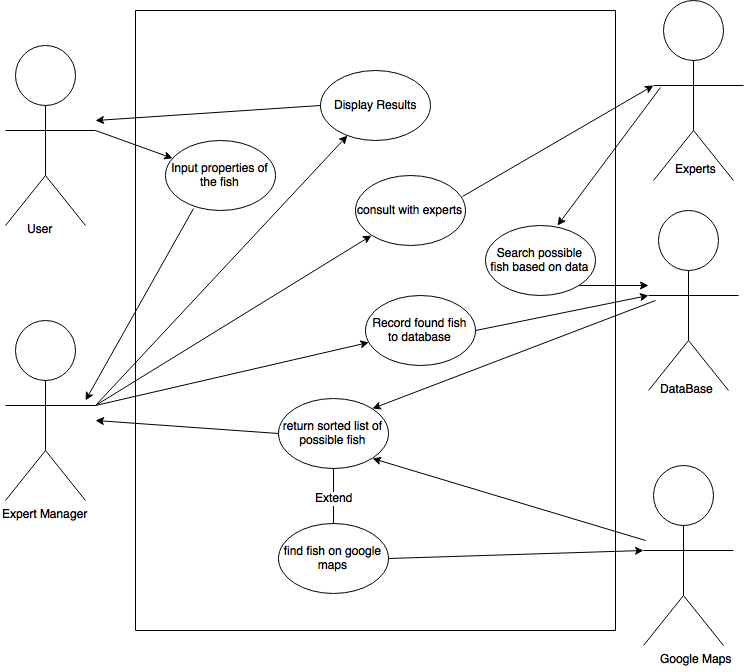
\includegraphics[width=\textwidth]{UseCase}
\caption{Use Case Diagram}
\end{figure}

\FloatBarrier

The following are brief descriptions of the Use Cases displayed above:
\begin{itemize}
\item \textbf{Input properties of fish:} \\
The user inputs the following attributes: Colour, pattern, place, and/or shape to the expert manager.
\item \textbf{Consult with experts:} \\
The expert manager inputs the attributes to a forum(blackboard). Experts will each grab their respective attributes to identify the fish.
\item \textbf{Search possible fish based on Data:} \\
The experts query the database to find possible fish that fit the attributes.
\item \textbf{Record found fish of database:} \\
The manager can choose to report found fish to the database of the application. Other users may view an estimate of the chances of finding this type of fish.
\item \textbf{Return sorted list of possible fish:} \\
A sorted list of possible fish from most to least probable will be returned to the forum.
\item \textbf{Find fish on google maps:} \\
The application may also display locations where this type of fish can be found.
\item \textbf{Display results:} \\
The returned result will be displayed to the user.
\end{itemize}
% End Section

\section{Analysis Class Diagram}
\label{sec:analysis_class_diagram}
% Begin Section
\begin{figure}
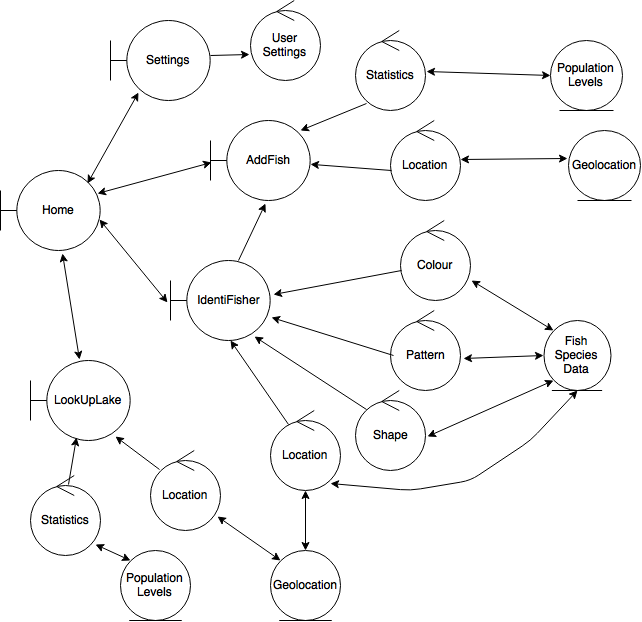
\includegraphics[width=\textwidth]{classAnalysis}
\caption{Class Analysis Diagram}
\end{figure}

\FloatBarrier

All boundary objects are connected to the home boundary object as that is where the users of the application will navigate from. Connected to the home boundary object are the main classes responsible for modifying user profile settings, identifying fish species, adding fish species to lake databases, and finding optimal fishing spaces in lakes. The classes are broken down to their respective control objects responsible for the many different options the users of the application will have access to. Each control object will be connected to their respective database sets which could include the population levels, geolocation, or data about different fish species.
% End Section

\section{Architectural Design}
\label{sec:architectural_design}
This section will outline a detailed description of the whole architecture system. This will include, but is not limited to, the name of the design, benefits of the design as well as a justification of the choice and enough detail to implement the design.

\subsection{System Architecture}
\label{sub:system_architecture}
This system will mainly consist of front end modules, processors, and entities.
The front end modules will consist of every view of the Android application. They will handle all the input from the user and output from the application. After accepting valid input from the user, the application will send that data to the processors. The processors will consist of the Experts and ExpertManager. They will process this information while querying the entities for information. The entities will consist of the Database used to store all information regarding the users and fish. After the processors are finished with the entities, the ExpertManager will return the processed information to the front end modules to be displayed. The front end modules will then display the information to the user and wait for more input. Due to this process, we will be using a Blackboard Architecture Style. The reasoning behind the choice is that all the experts are contributing to a single and complex problem. With a blackboard style architecture, all Expert modules can contribute as much as possible so the ExpertManager can make the best decision. Within the system, the ExpertManager will play the role of both the blackboard and controller, and the Expert modules will play the role of the knowledge source.

\begin{figure}
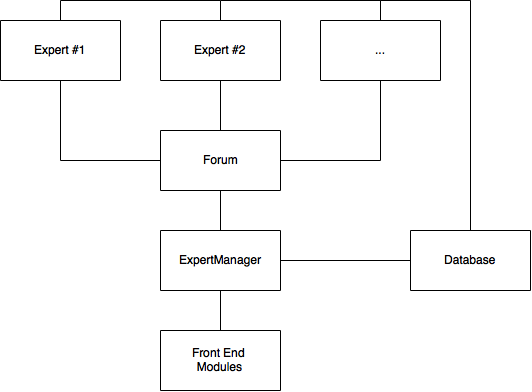
\includegraphics[width=\textwidth]{ArchDesign}
\caption{Graphical Representation of Architecture Deisgn}
\end{figure}

\FloatBarrier

\subsection{Subsystems}
\label{sub:subsystems}
This section serves the purpose of breaking each subsystem down and outlining the actions, responsiblites and expectations of each subsystem. Ordered with respect to level of abstraction, the following sections represent broad groupings each class will fall into. The following groups are as follows.
\subsubsection{Front End Modules}
These modules are majorly responsible for the input and output of the application. Without these being functional, it would be impossible for the user to interact with the application. It consists of all views in the Android Manifest and every element each view contains. It will perform minor data verification, provide ease of communication, and display an attractive, functional interface. The whole system depends on these modules to provide valuable, correct information so that it can process the information accordingly.
\subsubsection{Processors \& Controllers}
These modules are majorly responsible for the relay, delivery, and processing of all the information going through the application. Without these being functional, the front end modules would have no way of communicating to the data sources. It will perform the majority of the data verification, querying the database, and formatting the data returned.
\subsubsection{Data Source}
These modules are majorly responsible for holding all of the information in the application. This is necessary in order to use any information given by the user. It will perform organization, maintainance, and ensure the integrity of the information.

\section{Class Responsibility Collaboration (CRC) Cards}
\label{sec:class_responsibility_collaboration_crc_cards}

	\begin{table}[ht]
		\centering
		\begin{tabular}{|p{5cm}|p{5cm}|}
		\hline
		 \multicolumn{2}{|l|}{\textbf{Class Name: Home}} \\
		\hline
		\textbf{Responsibility:} & \textbf{Collaborators:} \\ \hline
		 This class is part of the front end modules and carries all the responsibilities associated with that. The responsibilities include handling all of the information coming from the user and displaying information to the user. This class in particular will be a hub to direct the user to the other front end modules. This class should be welcoming as it is the first thing the user will interact with.& It will collaborate with all the other front end modules. This is because it will provide the means for getting to the other modules. These include Settings, Look Up Lake and IdentiFisher. \\
		\hline
		\end{tabular}
	\end{table}

	\begin{table}[ht]
		\centering
		\begin{tabular}{|p{5cm}|p{5cm}|}
		\hline
		 \multicolumn{2}{|l|}{\textbf{Class Name: Settings}} \\
		\hline
		\textbf{Responsibility:} & \textbf{Collaborators:} \\ \hline
		 This class is part of the front end modules and carries all the responsibilities associated with that. These include handling all of the information coming from the user and displaying information to the user. This class in particular will be a hub to change any settings the user has that they have permissions for. & It will collaborate with the other front end modules and the Database. It needs to provide a means for getting to the other modules and change any settings that exist in the Database. \\
		\hline
		\end{tabular}
	\end{table}

	\begin{table}[ht]
		\centering
		\begin{tabular}{| p{5cm} | p{5cm} |}
		\hline
		 \multicolumn{2}{|l|}{\textbf{Class Name: LookUpLake}} \\
		\hline
		\textbf{Responsibility:} & \textbf{Collaborators:} \\ \hline
		This class is part of the front end modules and carries all the responsibilities associated with that. These include handling all of the information coming from the user and displaying information to the user. This class in particular will be a hub to look up statistics for fish that exist in a chosen lake. & It will collaborate with the other front end modules as well as the Database. It needs to provide a means for getting to the other modules and must be able to query the Database for information regarding each lake. \\
		\hline
		\end{tabular}
	\end{table}

	\begin{table}[ht]
		\centering
		\begin{tabular}{|p{5cm}|p{5cm}|}
		\hline
		 \multicolumn{2}{|l|}{\textbf{Class Name: IdentiFisher}} \\
		\hline
		\textbf{Responsibility:} & \textbf{Collaborators:} \\ \hline
		This class is part of the front end modules and carries all the responsibilities associated with that. These include handling all of the information coming from the user and displaying information to the user. This class in particular will be a hub to receive information from the user regarding a fish they would like to identify. & It will collaborate with the other front end modules and the processors. It needs to provide a means for getting to the other modules as well as send the information the user has provided to the processors in a useful way while maintaining data integrity. \\
		\hline
		\end{tabular}
	\end{table}

	\begin{table}[ht]
		\centering
		\begin{tabular}{|p{5cm}|p{5cm}|}
		\hline
		 \multicolumn{2}{|l|}{\textbf{Class Name: ExpertManager}} \\
		\hline
		\textbf{Responsibility:} & \textbf{Collaborators:} \\ \hline
		The ExpertManager is part of the processors and carries all the responsibilities associated with that. These include handling data verification and relaying information. This class in particular will get information from the IdentiFisher and update the Forum in a meaningful and accurate way. After the Forum has estimated what type of fish has been queried, the ExpertManager must read the Forum and relay the information back to the IdentiFisher class. & This class will work with the Forum and IdentiFisher.\\
		\hline
		\end{tabular}
	\end{table}

	\begin{table}[ht]
		\centering
		\begin{tabular}{|p{5cm}|p{5cm}|}
		\hline
		 \multicolumn{2}{|l|}{\textbf{Class Name: Forum}} \\
		\hline
		\textbf{Responsibility:} & \textbf{Collaborators:} \\ \hline
		The Forum is an entity/processor class and has most of the responsiblites for each type of class. The Forum will be updated by the ExpertManager which will allow the Expert modules to each add useful information to the problem being solved. Once the Forum has received all the information, it can be read by the ExpertManager to decide on a unique fish. & This class should be accessible only to the Expert and ExpertManager. \\
		\hline
		\end{tabular}
	\end{table}

	\begin{table}[ht]
		\centering
		\begin{tabular}{|p{5cm}|p{5cm}|}
		\hline
		 \multicolumn{2}{|l|}{\textbf{Class Name: Expert}} \\
		\hline
		\textbf{Responsibility:} & \textbf{Collaborators:} \\ \hline
		This class consists of many classes of Expert classes which are considered control classes, each bearing a separate and unique domain of expertise. The main responsibility is to read the Forum, gather information from it, and return the most probable fish that is attempting to be identified. Each Expert will work independently of the others. & These classes will all work separately with the Forum. \\
		\hline
		\end{tabular}
	\end{table}

	\begin{table}[ht]
		\centering
		\begin{tabular}{|p{5cm}|p{5cm}|}
		\hline
		 \multicolumn{2}{|l|}{\textbf{Class Name: Database}} \\
		\hline
		\textbf{Responsibility:} & \textbf{Collaborators:} \\
		\hline
		This class is an overall entity class which holds all the information the application needs to hold. This can hold user information, fish information, and statistics regarding lakes and the fish they contain. It is responsible for receiving, searching, and relaying information in a meaningful way while maintaining data integrity. & These classes will work with all other classes that need to get information that a particular class may hold. \\
		\hline
		\end{tabular}
	\end{table}

\FloatBarrier

\appendix
\section{Division of Labour}
\label{sec:division_of_labour}
% Begin Section
\begin{center}
\begin{tabular}{ |c|c|c| }
 \hline
 Name & Labour & Signature              \\ \hline
 Shani & Introduction & \\
 Chris & Class Responsibility Charts \& Architecture Design &  \\
 Ocean & Analysis Class Diagram &  \\
 Tian & Use Case Diagram & \\
 \hline
\end{tabular}
\end{center}

\newpage

\listoffigures

\end{document}
